\documentclass[12pt,letterpaper]{article}
\usepackage[utf8]{inputenc}

\usepackage[spanish, es-nodecimaldot]{babel}
\usepackage{amsmath}
\usepackage{color}
\usepackage{algorithm}
\usepackage[noend]{algpseudocode}
\renewcommand{\algorithmicrequire}{\textbf{Entrada:}}
\renewcommand{\algorithmicensure}{\textbf{Salida:}}
\usepackage{subcaption}
\usepackage{amsfonts}
\usepackage{hyperref}
 \hypersetup{
     colorlinks=true,
     linkcolor=blue,
     filecolor=blue,
     citecolor = blue,      
     urlcolor=cyan,
     }
\usepackage{amssymb}
\usepackage{listings}
\usepackage{color}

\definecolor{mygreen}{rgb}{0,0.6,0}
\definecolor{mygray}{rgb}{0.5,0.5,0.5}
\definecolor{mymauve}{rgb}{0.58,0,0.82}

\lstset{ 
  backgroundcolor=\color{white},   % choose the background color; you must add \usepackage{color} or \usepackage{xcolor}; should come as last argument
  basicstyle=\footnotesize,        % the size of the fonts that are used for the code
  breakatwhitespace=false,         % sets if automatic breaks should only happen at whitespace
  breaklines=true,                 % sets automatic line breaking
  captionpos=b,                    % sets the caption-position to bottom
  commentstyle=\color{mygreen},    % comment style
  deletekeywords={...},            % if you want to delete keywords from the given language
  escapeinside={\%*}{*)},          % if you want to add LaTeX within your code
  extendedchars=true,              % lets you use non-ASCII characters; for 8-bits encodings only, does not work with UTF-8
  firstnumber=1,                % start line enumeration with line 1000
  frame=single,	                   % adds a frame around the code
  keepspaces=true,                 % keeps spaces in text, useful for keeping indentation of code (possibly needs columns=flexible)
  keywordstyle=\color{blue},       % keyword style
  language=Octave,                 % the language of the code
  morekeywords={*,...},            % if you want to add more keywords to the set
  numbers=none,                    % where to put the line-numbers; possible values are (none, left, right)
  numbersep=5pt,                   % how far the line-numbers are from the code
  numberstyle=\tiny\color{mygray}, % the style that is used for the line-numbers
  rulecolor=\color{black},         % if not set, the frame-color may be changed on line-breaks within not-black text (e.g. comments (green here))
  showspaces=false,                % show spaces everywhere adding particular underscores; it overrides 'showstringspaces'
  showstringspaces=false,          % underline spaces within strings only
  showtabs=false,                  % show tabs within strings adding particular underscores
  stepnumber=2,                    % the step between two line-numbers. If it's 1, each line will be numbered
  stringstyle=\color{mymauve},     % string literal style
  tabsize=2,	                   % sets default tabsize to 2 spaces
  title=\lstname                   % show the filename of files included with \lstinputlisting; also try caption instead of title
}

\usepackage{amsthm}
\newtheorem{theorem}{Teorema}

\usepackage{graphicx}
\usepackage[left=2cm,right=2cm,top=2cm,bottom=2cm]{geometry}
\setlength{\parskip}{3mm}
\title{\textsc{Teorema de Bayes}}
\author{\textsc{Fabiola Vázquez}}

\setlength{\parindent}{0cm}
\renewcommand{\lstlistingname}{Código}
\floatname{algorithm}{Algoritmo}

\begin{document}
\maketitle

\hrule
\section{Introducción}
El objetivo de este estudio es trabajar con el \textit{teorema de Bayes} y su aplicación en la interpretación de las pruebas diagnósticas de COVID-19. 

\section{Análisis}
Cuando se realiza un tipo de prueba, se espera saber con certeza si el paciente está enfermo o no, pero dado que ninguna prueba es perfecta, puede haber errores. En particular, hay cuatro tipos de resultados posibles, que están descritos en el cuadro \ref{resultados}. 

Los valores que representan los aciertos de las prueba son la sensibilidad, $P(+\mid \text{Enfermo})$, y la especificidad, $P(-\mid \text{No enfermo}).$ A partir de estos, otro tipo de valores se pueden obtener con el \textit{teorema de Bayes} (teorema \ref{thm}), como lo son $P(\text{Enfermo} \mid +)$ y $P(\text{No enfermo} \mid -)$.
\begin{table}
\centering
\caption{Diferentes tipos de resultados en una prueba.}
\begin{tabular}{|c|c|c|}
\hline 
Resultado & No enfermo & Enfermo \\ 
\hline 
+ & Falso positivo &  Verdadero positivo \\ 
\hline 
$-$ &  Verdadero negativo & Falso negativo  \\ 
\hline 
\end{tabular} 
\label{resultados}
\end{table}

\begin{theorem} \label{thm}
Sea $B_1, B_2, \ldots$ una partición del espacio muestral tal que $P(B_i)>0$, para toda $i$, y $A$ un evento cualquiera con probabilidad positiva, entonces 
\begin{equation} 
P(B_i \mid A) = \frac{P(A \mid B_i ) P(B_i)}{\sum^\infty_{j=1} P(A \mid B_j) P(B_j)}.
\end{equation}
\end{theorem}

Por el teorema anterior, se tiene que
\begin{equation} \label{p_cond}
P(\text{Enfermo} \mid +) = \frac{P(+ \mid \text{Enfermo})\times P(\text{Enfermo})}{P(+\mid \text{Enfermo}) \times P(\text{Enfermo})+P(+\mid \text{No enfermo}) \times P(\text{No enfermo})},
\end{equation}
donde $P(+\mid \text{Enfermo})$ es la sensibilidad y $P(+\mid \text{No enfermo})$ es igual a $1-$especificidad. Reescribiendo la ecuación \ref{p_cond}, se tiene
\begin{equation}
P(\text{Enfermo} \mid +) = \frac{\text{sensibilidad} \times P(\text{Enfermo})}{\text{sensibilidad} \times P(\text{Enfermo})+(1-\text{especificidad})\times (1 - P(\text{Enfermo}))}.
\end{equation}

\subsection{COVID-19}
En el estado de Nuevo León, se han realizado un total de 233,412 pruebas, resultando 78,389 de estas positivas y 155,023 negativas \cite{nl}. Según los indicadores del gobierno \cite{indicadores_nl}, en promedio un 40\% de las pruebas salen positivas. 

En el cuadro \ref{cov1} se considera la realización de 233,410 pruebas, con una sensibilidad del 80\%, una especificidad del 97.5\% y una probabilidad marginal de tener COVID-19 del 40\%. Esto lleva a los resultados mostrados, cuyos valores se aproximan a los reales. Además, con dichos datos se calcula la probabilidad $P(\text{Enfermo} \mid +)$ y se obtiene que la probabilidad de estar enfermo, dado que la prueba de COVID-19 salió positiva, es de 95.5\%.

Si por el contrario consideramos la probabilidad de tener COVID-19 como la cantidad de casos confirmados entre la población total de 5.12 millones, tendríamos una probabilidad marginal del 1\%. Si además se asume una sensibilidad  y una especificidad del 90\%, la $P(\text{Enfermo} \mid +)$ cambia y ahora se tiene una probabilidad del 8.3\%.

Para analizar las variaciones de $P(\text{Enfermo} \mid +)$, se consideran distintos valores de $P(\text{Enfermo})$ y se varía el valor de la sensibilidad o de la especificidad de la prueba. Dicho experimento se realiza en el software R \cite{R} en un cuaderno de Jupyter \cite{jupyter}, y los resultados se observan en las figuras \ref{especificidad} y \ref{sensibilidad}.  
\begin{table}
\centering
\caption{Datos obtenidos asumiendo sensibilidad del 80\% y especificidad del 97.5\%.}
\begin{tabular}{|c|r|r|r|}
\hline 
Resultado & No enfermo & Enfermo & Total\\ 
\hline 
+ & 74,691 & 3,501 & 78,192  \\ 
\hline 
$-$ & 18,672 & 136,546 & 155,218\\ 
\hline 
Total & 93,363 & 140,047 & 233,410\\
\hline
\end{tabular} 
\label{cov1}
\end{table}

\begin{figure}
 	\centering 
 	\begin{subfigure}[b]{0.45\linewidth}
 		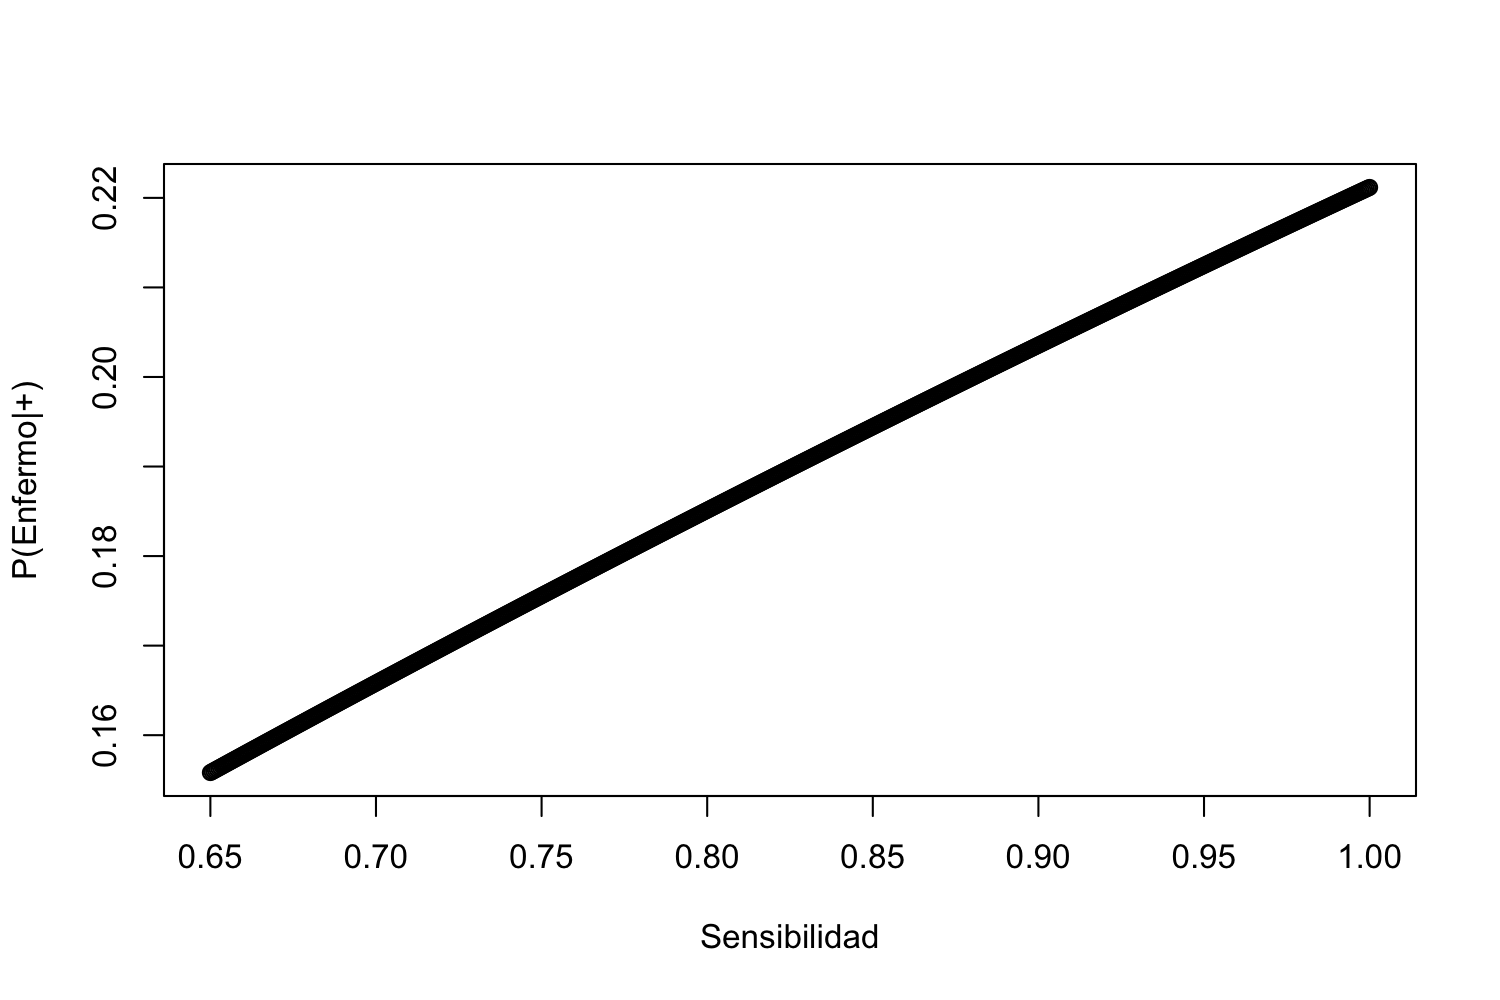
\includegraphics[width=\linewidth]{p1_sens.png} 		
 		\caption{$P(\text{Enfermo})=0.01$.}
 		 		\label{cuadratica}
 	\end{subfigure}
 	\begin{subfigure}[b]{0.45\linewidth}
 		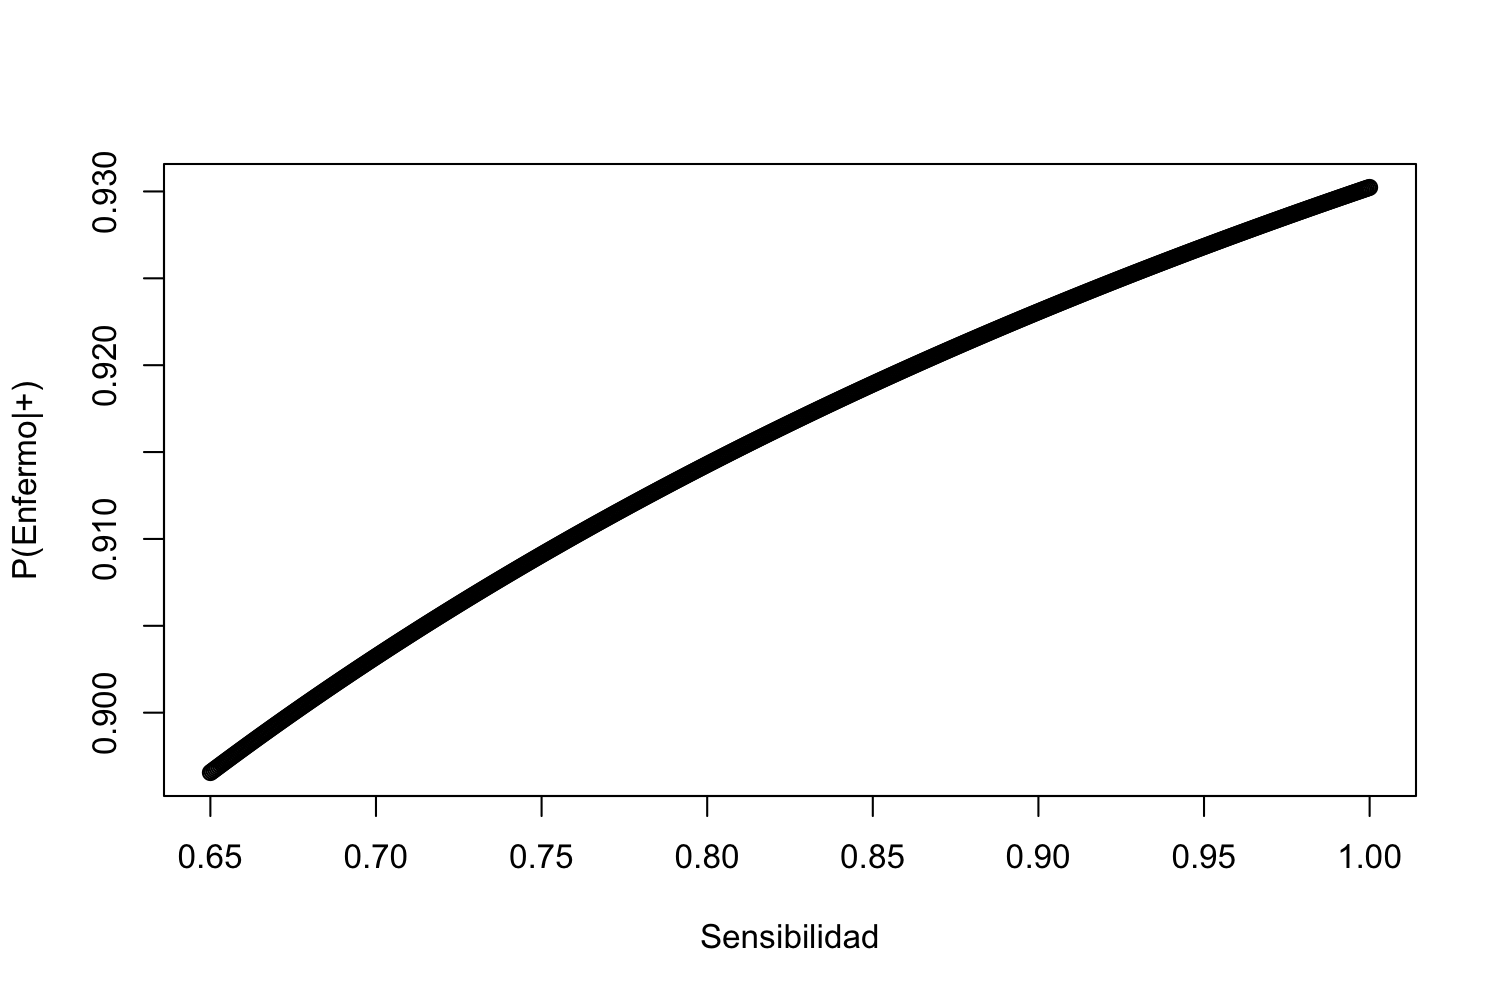
\includegraphics[width=\linewidth]{p2_sens.png} 		
 		\caption{$P(\text{Enfermo})=0.4$.}
 	\end{subfigure}
 	\begin{subfigure}[b]{0.45\linewidth}
 		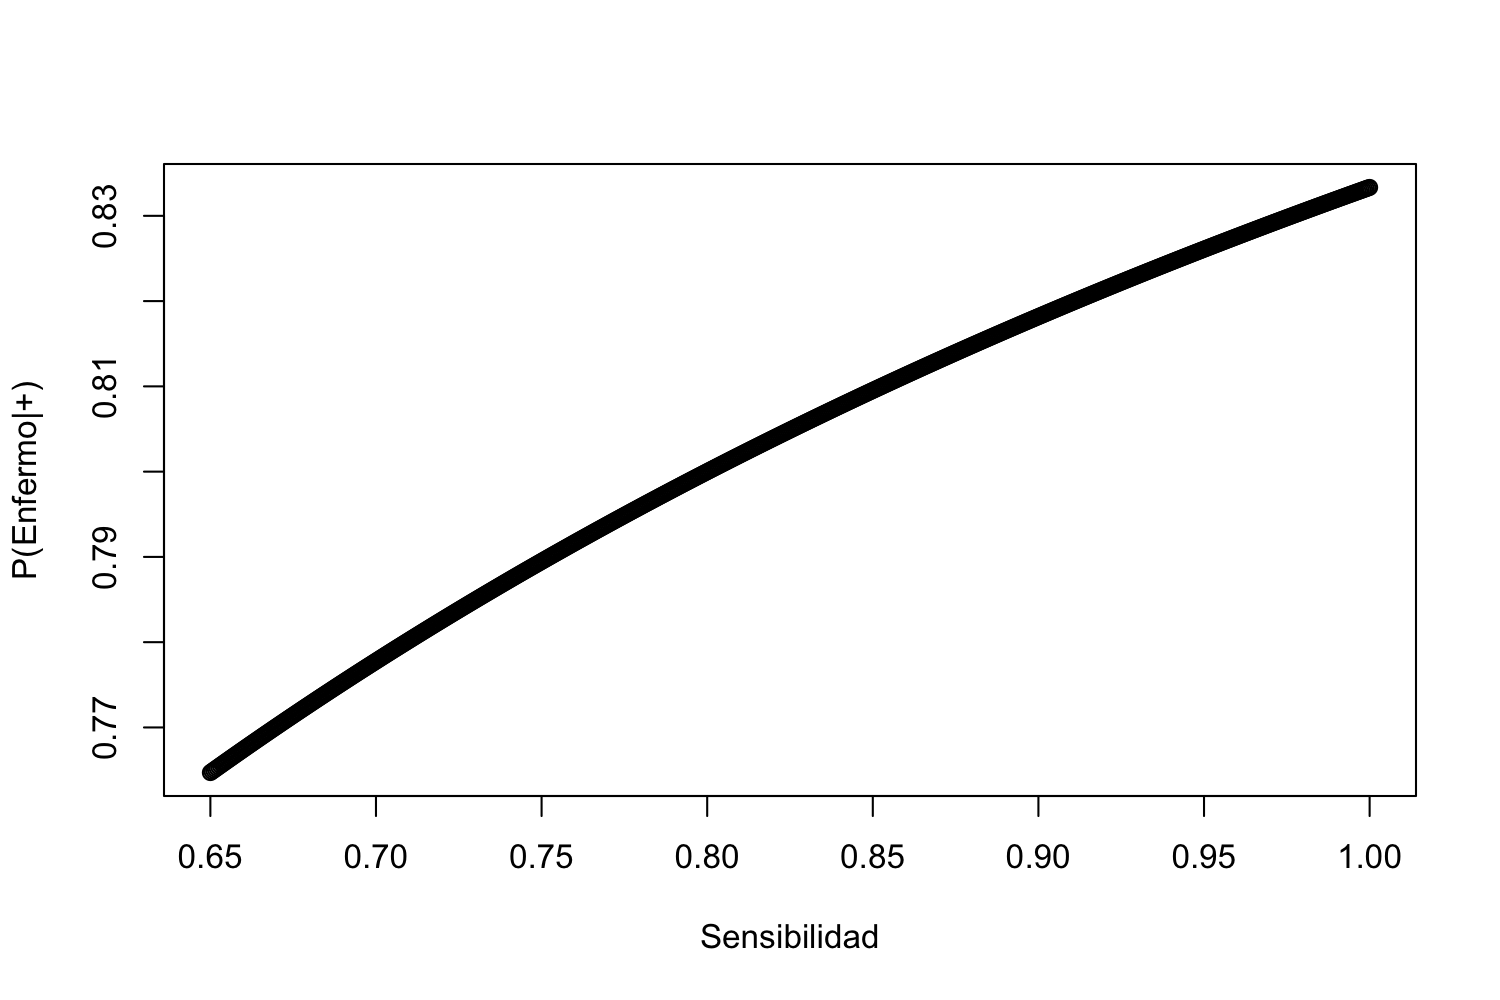
\includegraphics[width=\linewidth]{p3_sens.png} 		
 		\caption{$P(\text{Enfermo})=0.2$.}
 	\end{subfigure}
 	\begin{subfigure}[b]{0.45\linewidth}
 		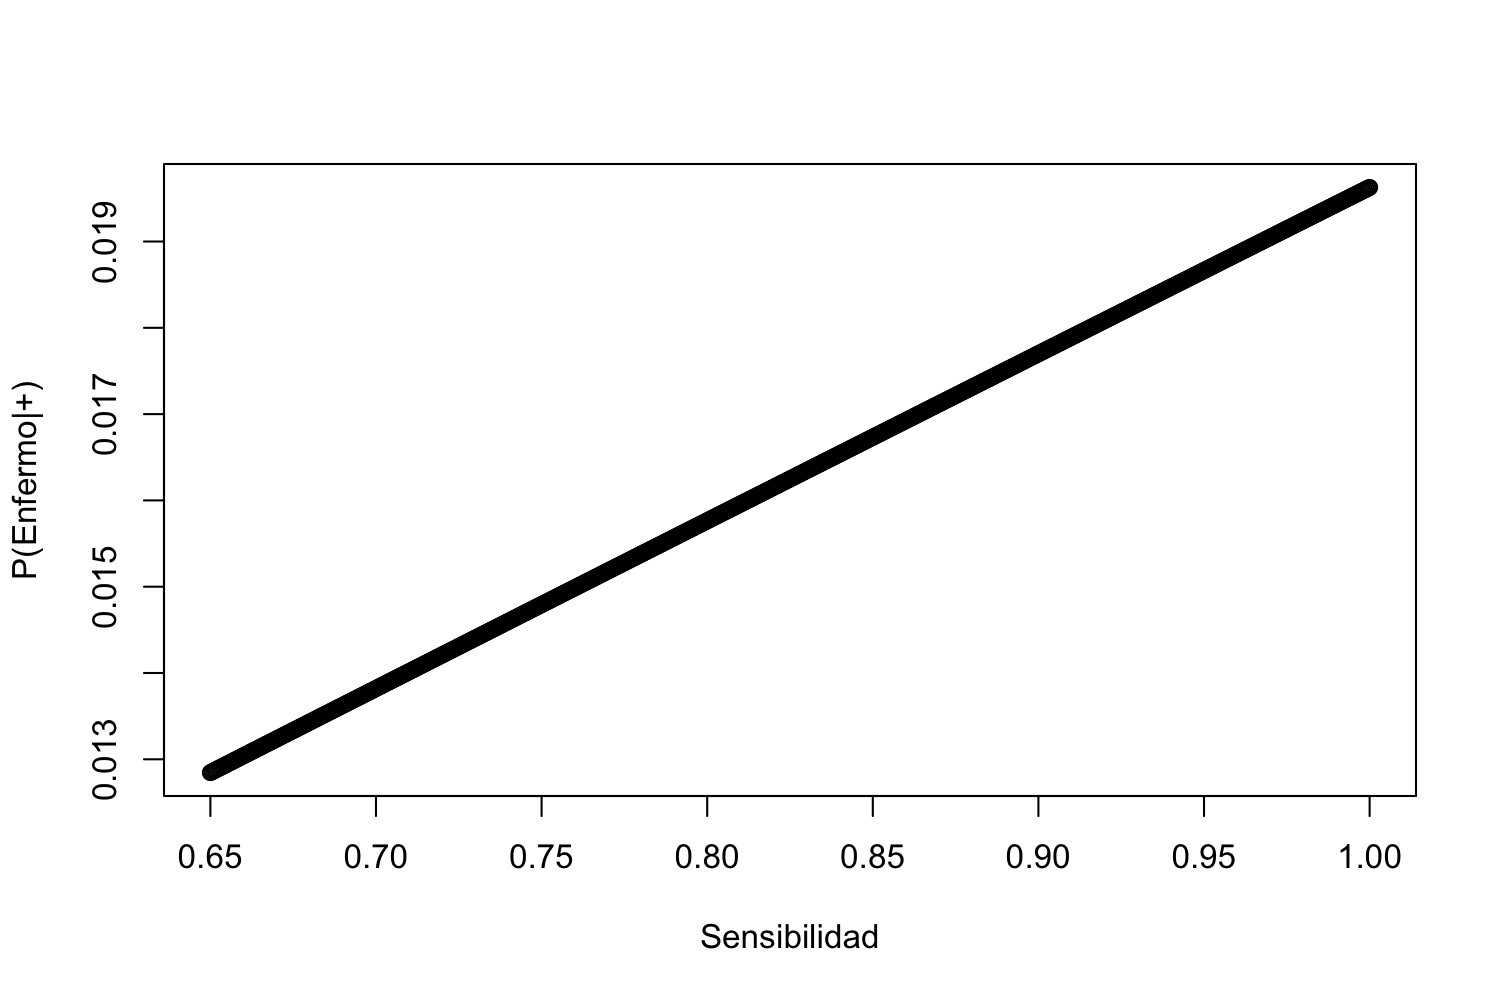
\includegraphics[width=\linewidth]{p4_sens.png} 		
 		\caption{$P(\text{Enfermo})=0.001$.}
 	\end{subfigure}
 	 	\caption{Considerando la especificidad como el 95\%.}
 	 		\label{especificidad}
\end{figure}

\begin{figure}
 	\centering 
 	\begin{subfigure}[b]{0.45\linewidth}
 		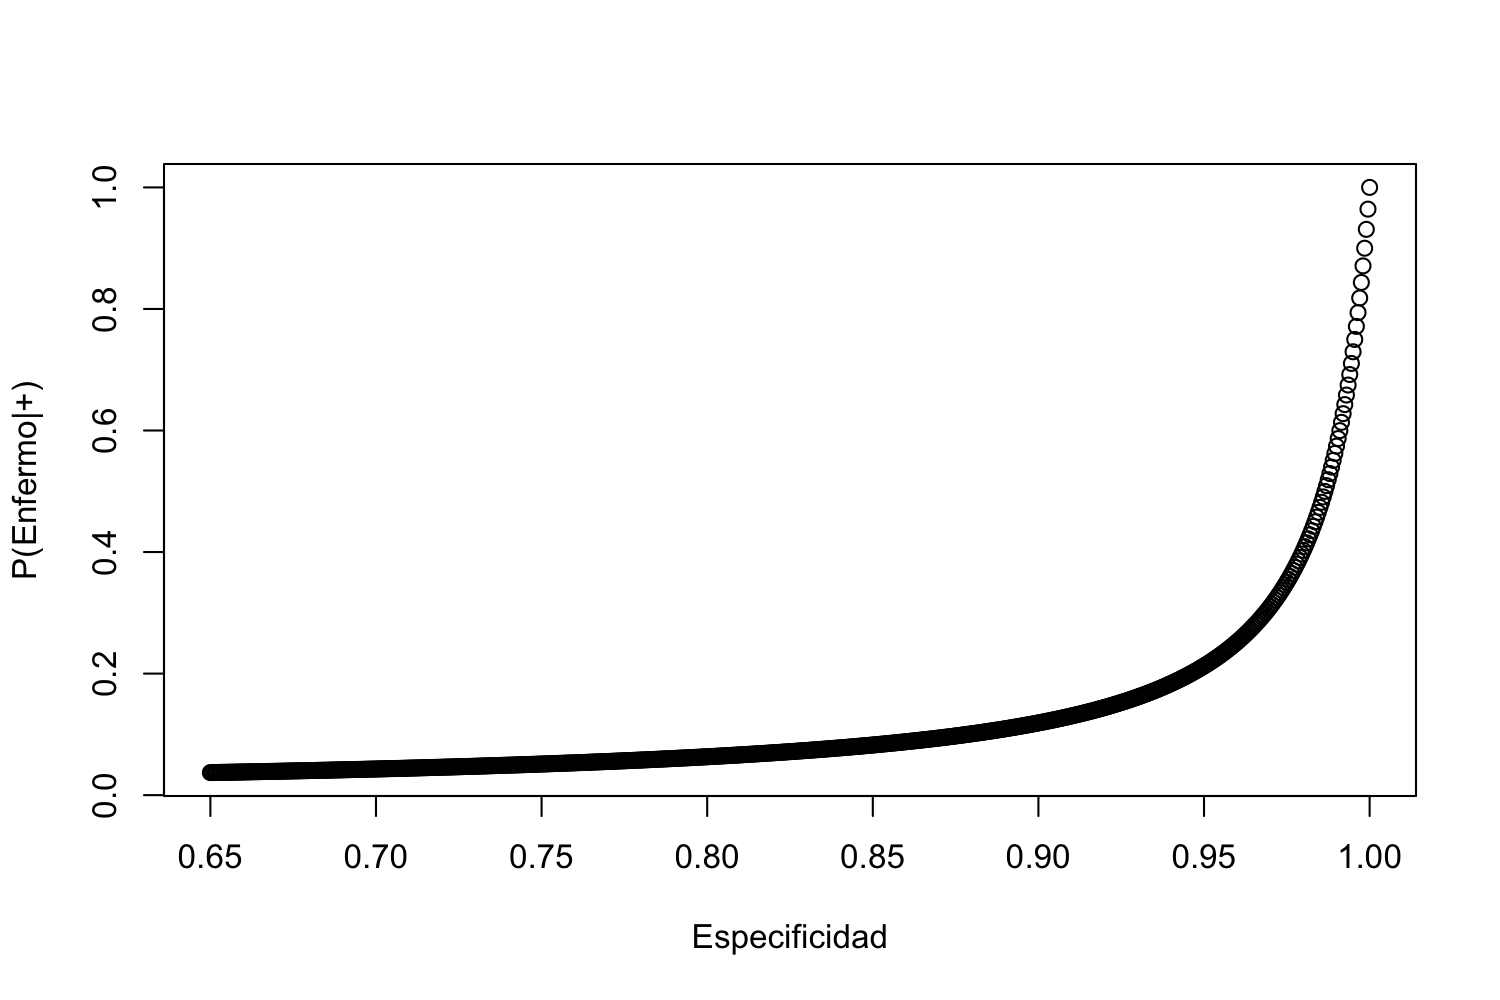
\includegraphics[width=\linewidth]{p1_spec.png} 		
 		\caption{$P(\text{Enfermo})=0.01$.}
 	\end{subfigure}
 	\begin{subfigure}[b]{0.45\linewidth}
 		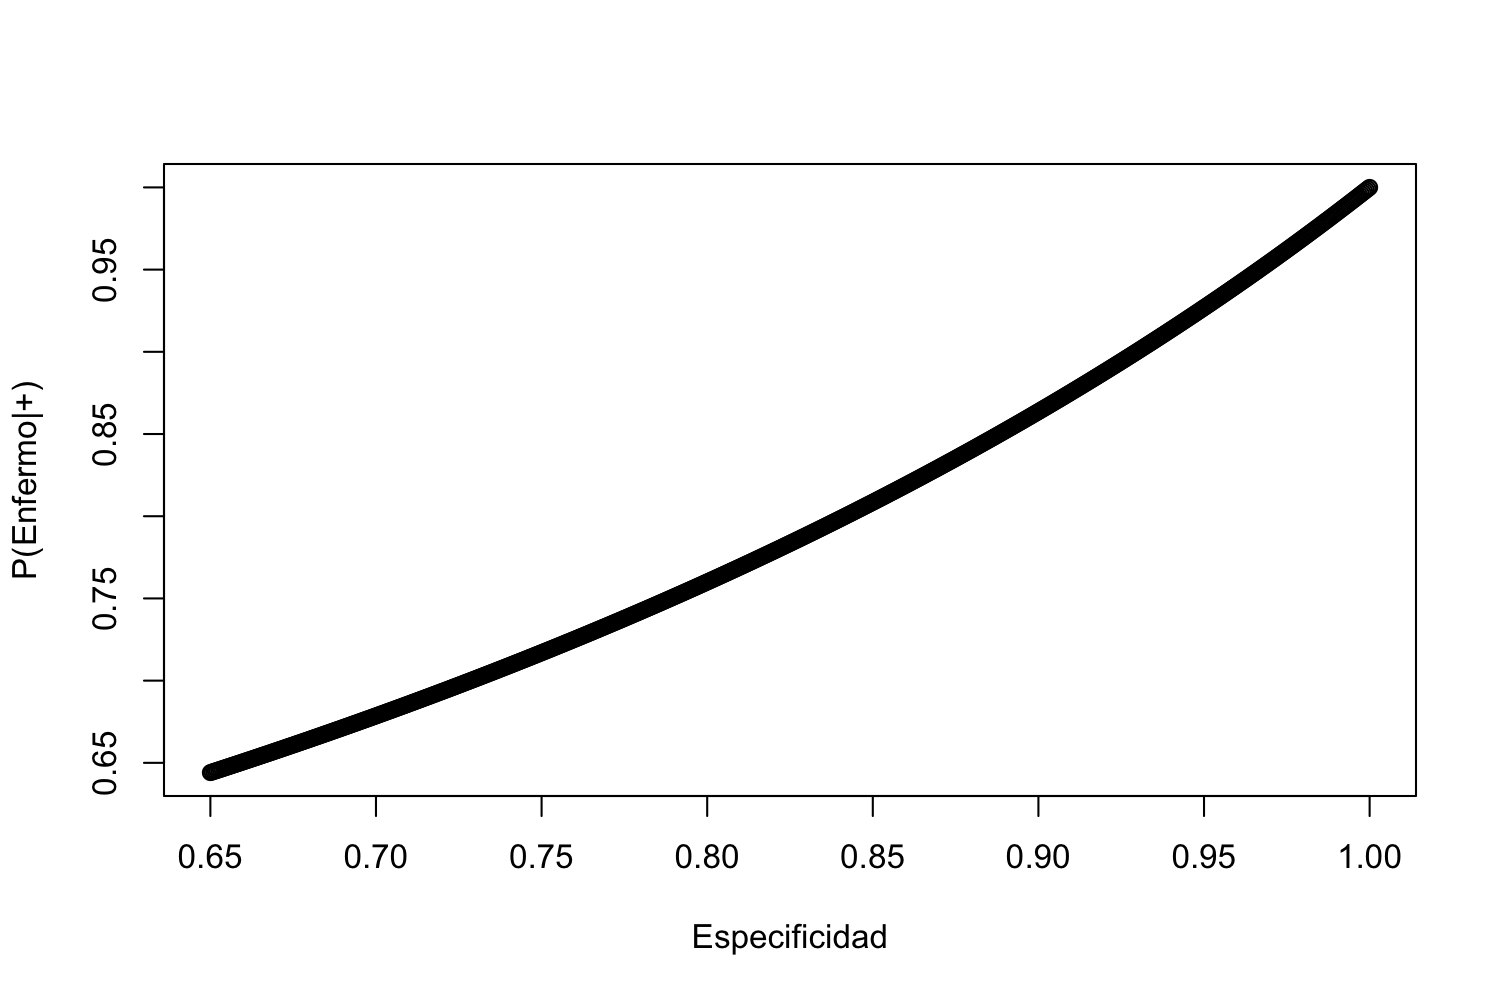
\includegraphics[width=\linewidth]{p2_spec.png} 		
 		\caption{$P(\text{Enfermo})=0.4$.}
 	\end{subfigure}
 	\begin{subfigure}[b]{0.45\linewidth}
 		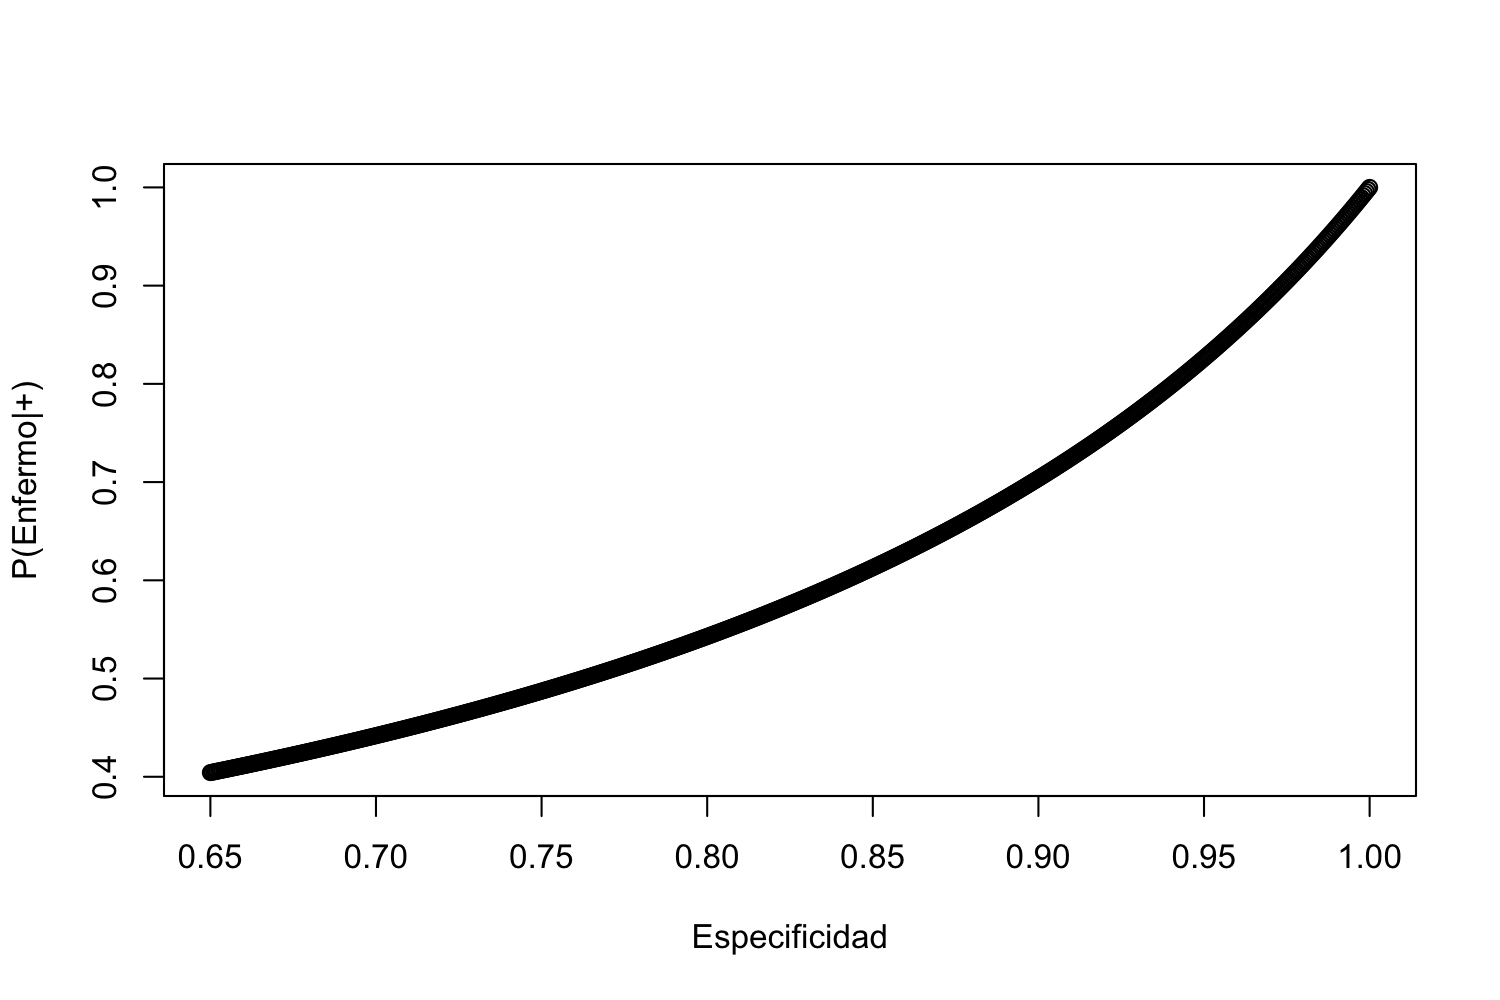
\includegraphics[width=\linewidth]{p3_spec.png} 		
 		\caption{$P(\text{Enfermo})=0.2$.}
 	\end{subfigure}
 	\begin{subfigure}[b]{0.45\linewidth}
 		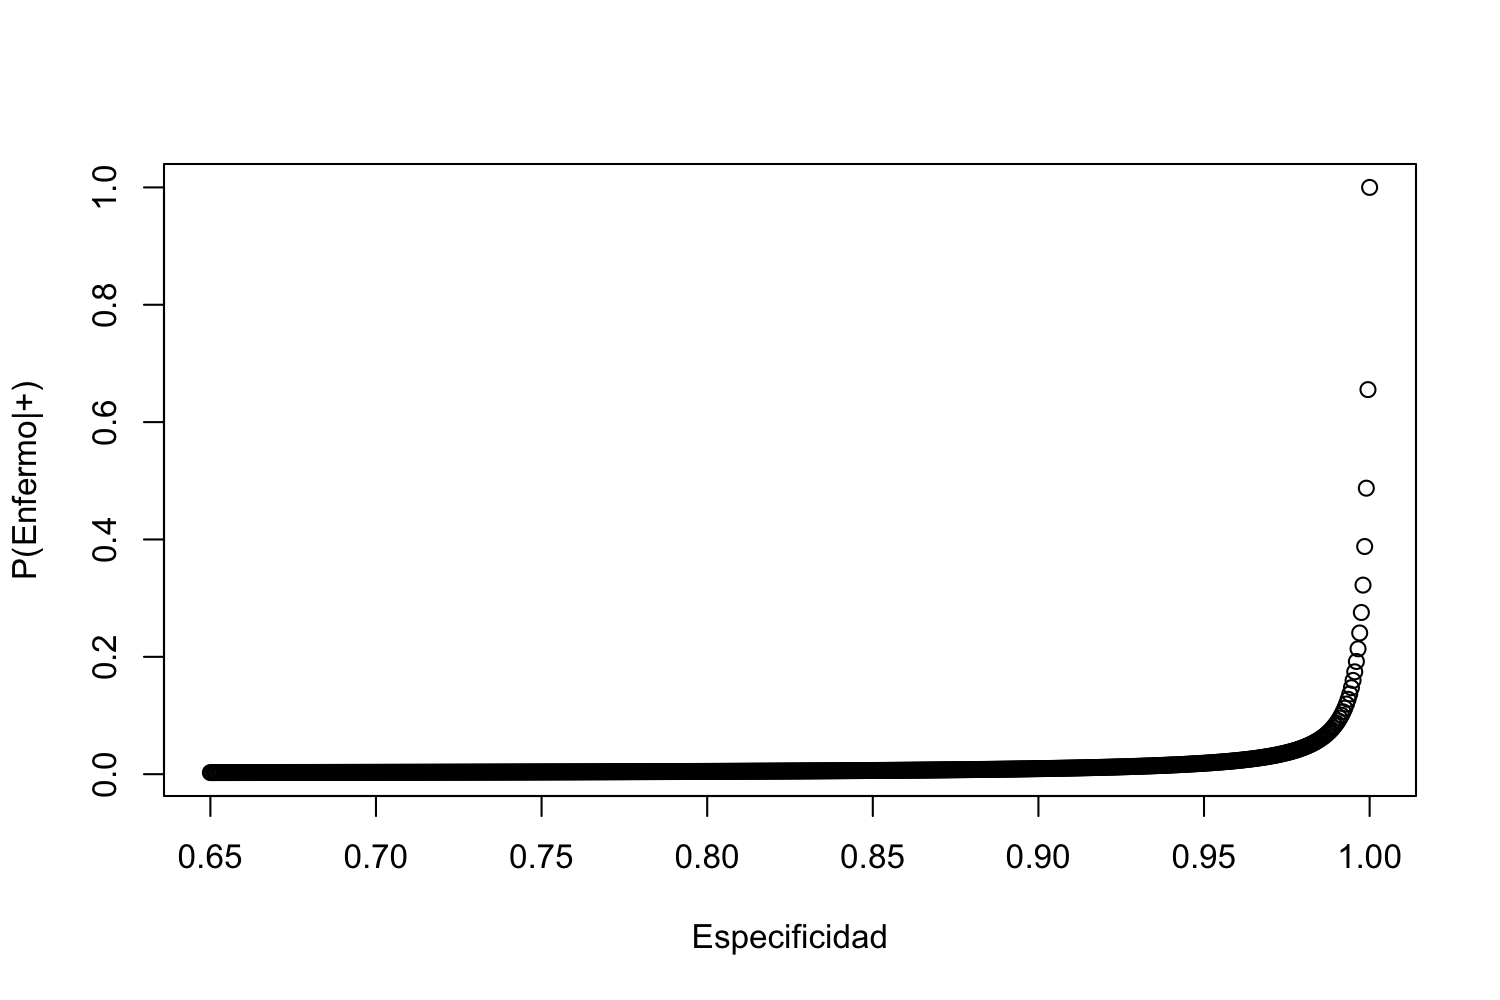
\includegraphics[width=\linewidth]{p4_spec.png} 		
 		\caption{$P(\text{Enfermo})=0.001$.}
 	\end{subfigure}
 	 	\caption{Considerando la sensibilidad del 95\%.} 
 	 		\label{sensibilidad}
\end{figure}

\subsection{Influenza}
Con la temporada de influenza acercándose, y dada la similitud de sus síntomas con los del COVID-19, será de particular importancia distinguir entre estas enfermedades. De acuerdo con los datos del CDC, las pruebas rápidas de influenza tienen una sensitividad de 50\% a 70\%, y una especificidad de 90\% a 95\% \cite{flu_ridt_cdc}. En el invierno 2018-2019, se estimaron 36 millones de casos de influenza en EE. UU.  \cite{flu_burden_cdc}, con una población de 329 millones \cite{us_pop_clock}. Con los datos mencionados, se tendría $P(\text{Enfermo}) = 36/329 \approx 0.10$, y una probabilidad condicional que va de $P(\text{Enfermo}|+) = .35$ a $P(\text{Enfermo}|+) = .60$.

\bibliographystyle{plain} 
\bibliography{Ref}


\end{document} 